\chapter{Feature selection}

In order to create an effective predictive model one must first select a set of features used to produce each classification. Both a science and an art, this process involves intuition, theory and a hefty amount of trial-and-error. Although a seemingly daunting task, for a model to be effective the feature selection procedure is key, and a carefully considered selection often generates significantly better results than one hastily put together. 

Ideally, one seeks a small set of variables which accurately captures the information content in a larger set of data. After reducing the number of features into a more manageable format it is then possible to obtain good results with significantly less computational load than if no feature selection had been considered. Furthermore, the feature selection process allows us to pinpoint what data characteristics we wish to monitor, and subsequently which data characteristics we can disregard. 

\section{An impossible problem}

Fundamentally, the radar used transmits pulses with some envelope $A(t)$ of some frequency $\Omega$ into its surroundings.

\begin{equation}
	x(t) = A(t)\sin(\Omega t + \varphi)
\end{equation}

After scattering, a signal $s(t)$ reaches the receiving antenna. This signal is comprised of radiation diffuesly scattered from the target scene. It contains both specular (i.e. mirror-like) and non-specular reflective components. Its content will be a function dependant both on the surrounding surface topography, as well as the dielectric properties of the surface at hand \citep{grossman_popovic_chamberlin_gordon_novotny_2017}. Furthermore, the surfaces at hand have a, to some degree, random structure with varying properties. The great difficulty with modeling $s(t)$ is clear - the universe of all possible "realistic" surfaces, both natural and man-made, is almost impossibly large. And since we in the present case are unable to make any significant assumptions with regards to the surface landscapes tested, there is no real useful model of $s(t)$ we can make. Instead, we have to come up with a set of \emph{reasonable} features that \emph{should} capture the signal structure. Hence our task is to find \emph{defining characteristics} from a given surface using the sequence of one dimensional data obtained from a radar sensor. 

The reflectivity of a material, described by its dielectric constant, shows up in the obtained IQ-demodulated sweeps in the amplitude of the returning signals. Therefore it might seem like a good idea to simply measure the energy content of a sweep and use it as a feature. However, due to inconsistencies inbetween individual sensors sweep normalization is performed as a pre-processing step rendering such calculations unusable. We are thus left with investigating the topography of the scene. 

As the radar samples rather quickly at around 200 Hz we can allow ourselves to use a sequence of sweeps to generate one prediction. This allows for feature-processing over a number of sweeps, rather than on a sweep-by-sweep basis. Besides improving the signal-to-noise ratio \citep{w_doerry_2016} we may also investigate time correlations when using multiple radar sweeps. If $T$ sweeps are used per classification, the rate of classifications $F_c$ produced relates to the sampling rate $F_s$ through

\begin{equation}
	F_c = \frac{F_s}{T}
\end{equation}

The parameter $T$ becomes a tradeoff between accuracy and classification rate. The more samples $T$ used per classification the higher the classification accuracy is at the cost of a lower classification frequency. Conversely we may be able to generate feature estimates more rapidly by setting $T$ to a lower value, but will in the process end up with worse feature estimates. 

\section{Features}

In this section four different features are discussed aimed at capturing the geometric characteristics of a target surface. A radar datapoint captured at time $t$ and range $n$ is denoted as $x(n,t)$. Since we are using $T$ samples per classification, each new set of features $f_m$ are estimated from time $t_m=Tm$ to $Tm+T-1$ 

\subsubsection{Expected signal}

First of all we may characterize a sweep by its envelope form - that is, the shape of the absolute values of the radar sweeps. For range $i$ and features $m$, $T$ consecutive samples are averaged over to yield the estimate. 

\begin{equation}
	s_i(m) = \E\{X_{i,t_m}\} = \frac{1}{T}\sum_{t=0}^{T-1}x(i, t_m + t).
\end{equation}

\begin{figure}[h]
	\centering
	\includegraphics[scale=0.7]{figs_temp/features/sweep_average}
	\caption{By averaging a number of consecutive sweeps, we reduce noise and make samples more similar. The dashed line shows the average of the solid lines. }
	\label{fig:sweep_average}
\end{figure}

\subsubsection{Average energy}
The average energy in a sweep tells us how much energy is reflected back to the radar. Hence it can be regarded as a measure of how good of a reflector the underlying surface is. The energy depends on the shape of the surface, as well as its dielectric constant. Compared to other materials, grass has a very different surface shape, which potentially gives it a very different reflexivity. However, its dielectric constant could also vary a lot depending on whether it is wet or dry, making it hard to guess its reflective properties.

By computing the average energy of single sweeps from different surfaces we see in figure \ref{fig:sweep_energy} that grass reflects much less energy. This indicates that the average sweep energy is a good feature for binary grass/not grass classification. However, in order to get a more robust measure of the average energy we do not only compute the average over selected range bins of a single sweep, but we average over a few consecutive sweeps as well. Mathematically, the feature we end up using becomes
\begin{equation}
	P(t_m) = \frac{1}{NT}\sum_{t=0}^{T-1}\sum_{n=0}^{K-1}x(n, t_m + t)x^*(n, t_m + t),
\end{equation}
where (describe variables)

Despite the fact that the average energy appears to be a highly relevant feature, it is also much gain dependent, and conflicts with what is stated in section *reference to sweep norm.*. Therefore, if different sensors are to be used for training and future classifications, this feature will not be of any use.

\begin{figure}[h]
	\centering
	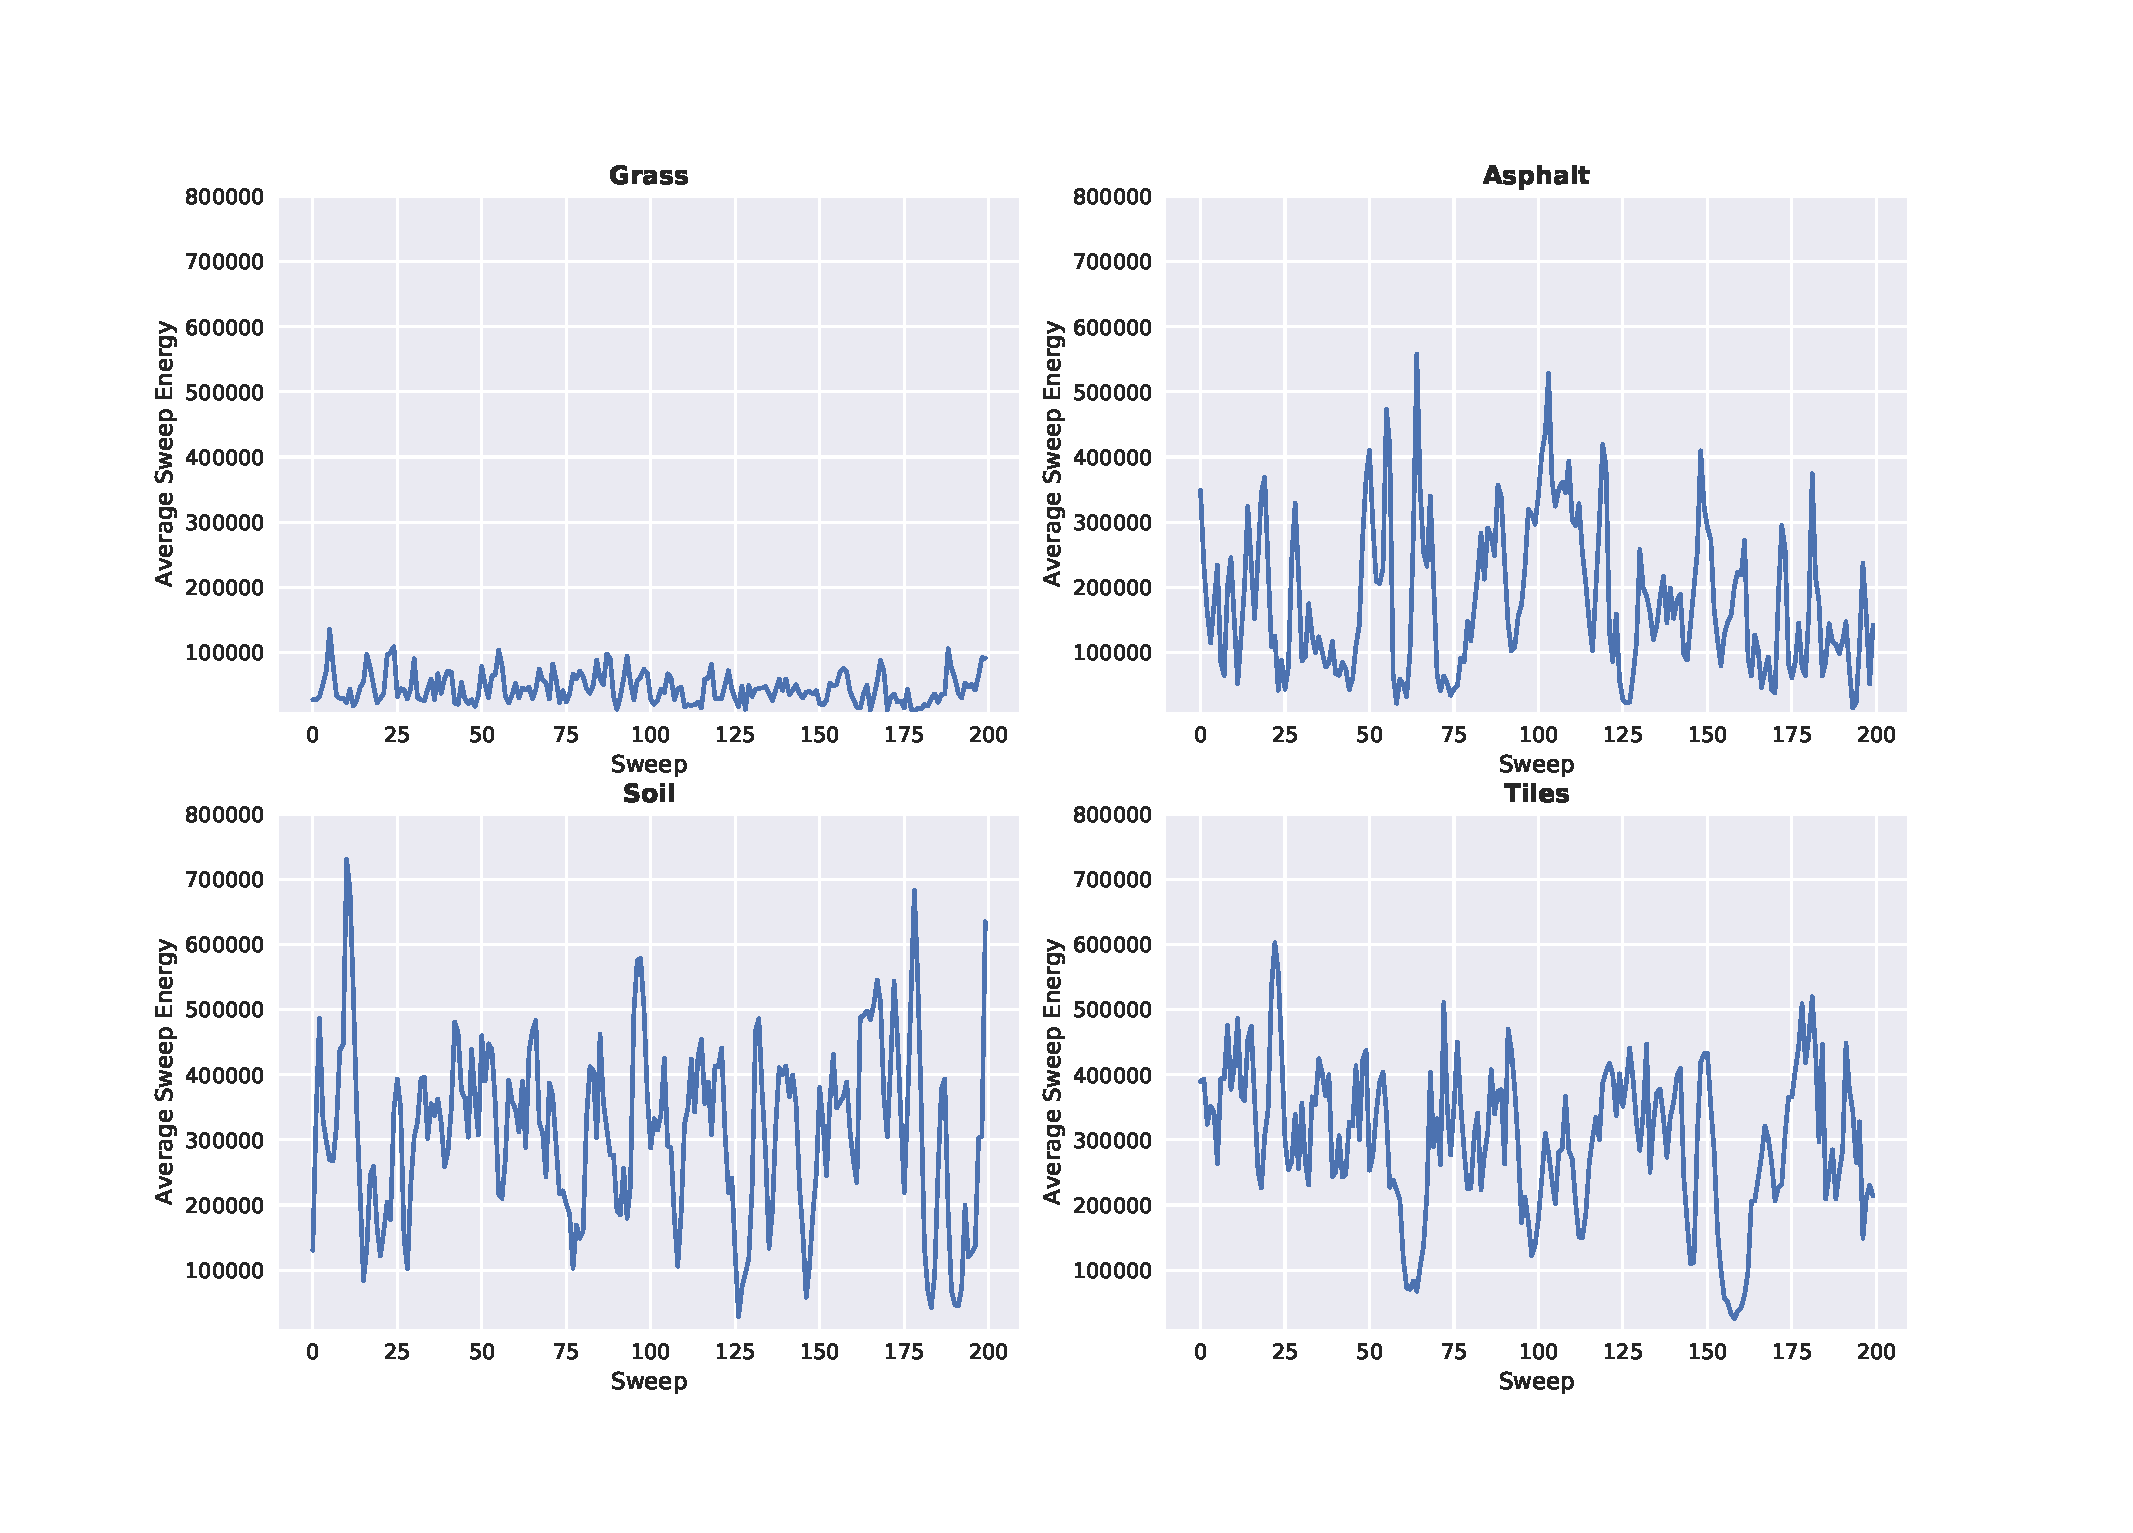
\includegraphics[scale=0.45]{figs_temp/features/sweep_energy}
	\caption{The figure shows the average sweep energy for 200 sweeps and four different materials. All measurements were made during a short period of time. The reflections from the grass surface carry noticeably less energy than those from the other surfaces. }
	\label{fig:sweep_energy}
\end{figure}



\subsection{Fourier Transform}
The surface underneath the radar can be assumed to be static, whereas the radar traverses the surface at a constant speed. This causes the radar to detect doppler frequencies. Depending on the surface's characteristics, the doppler frequencies may vary, (according to figure *Figure comparing reflections on a flat and rough terrain*?) and to visualize the frequency contents of different measured materials, the discrete Fourier transform is used. 

To compute the Fourier transform, a "box" consisting of $T$ sweeps is selected. Viewing this as a matrix with elements $X_{n,t}$, where $n$ denotes slow time, and $t$ fast time we can write a Fourier transform in slow time at range $r$, within this box as
\begin{equation}
	\mathbb{X}_k^{(r)} = \sum_{n=0}^{T-1}X_{n,r}\exp\Big[-2\pi i\frac{nk}{T}\Big] \quad k=0, ..., T-1.
\end{equation}
In figure \ref{fig:fft} five consecutive 128-step Fourier transforms have been computed for four materials. For grass (top plot), it can be seen that the frequency content is contained mainly at the start of the "FFT blocks", which corresponds to normalized frequency 0. The other materials contain slightly higher frequency content as well.

To avoid aliasing we refer to chapter earlier in report where this is discussed. Mention that $\mathbb{X}_k^{(r)}$, for all $r$, $k$, is flattened to a vector, resulting in one new sample.

\begin{figure}[h]
	\centering
	\includegraphics[scale=0.4]{figs_temp/features/fft}
	\caption{Each plot shows 5 concatenated DFTs, which have all been estimated from 128 consecutive sweeps. This has been done for ranges 7-23 cm, and the materials included in the figure are grass, asphalt, soil and tiles, respectively. Each FFT box has an $x$-axis going from normalized frequency 0 to 1.}
	\label{fig:fft}
\end{figure}




\subsection{Variance}

Assume $x(n,t)$ are samples from a complex normal distribution $X_{n,t}$. Variance $v_i(t_m)$ at range $i$ at time $t_m$ can then be approximated using

\begin{equation}
\label{eq:var}
\begin{gathered}
	v_i(t_m) = \E\{ (X_{i,t_m} - \E\{X_{i,t_m}\})^2\} \\
	= \frac{1}{T-1}\sum_{t=0}^{T-1}(x(i, t_m + t) - s_i(t_m))^*(x(i, t_m + t) -  s_i(t_m))
\end{gathered}
\end{equation}

\subsection{Autocovariance in slow time}

\textbf{Add some motivation for using autocovariance}

\noindent
For some stochastic process $P_t$ we can define the autocovariance $\gamma$ as

\begin{equation}
	\gamma(t, s) = \E\big\{(P_t - \mu_t)(P_s - \mu_s)\big\}
\end{equation}

If $X_t$ is a weakly stationary process the first moment (mean) and autocovariance do not vary over time.  The autocovariance then only depends on the difference between $s$ and $t$, making it possible to rewrite as

\begin{equation}
	\gamma(\tau) = \E\big\{(P_t - \mu)(P_{t+\tau} - \mu)\big\}
\end{equation}

Assuming weak stationarity over a few rangebins we can estimate the autocovariance in slow time for each selected range. 

\begin{equation}
\begin{gathered}
	\gamma_i(t_m, \tau) = \E\big\{(X_{i,t_m} - \E\{X_{i, t_m}\})^*(X_{i, t_m+\tau} - \E\{X_{i, t_m+\tau}\})\big\}\\
	= \frac{1}{T-1}\sum_{t=0}^{T-1-\tau}(x(i, t_m + t) - s_i(t_m))^*(x(i, t_m + t + \tau) - s_i(t_m + \tau))
\end{gathered}
\end{equation}•

We can drop the $\tau$ in the final expectation term, as $s_i(t)$ are estimated in batch from $t_m$ to  $t_m + T$ yielding

\begin{equation}
	\gamma_i(t_m, \tau) = \frac{1}{T-1}\sum_{t=0}^{T-1- \tau}(x(i, t_m + t) - s_i(t_m))^*(x(i, t_m + t + \tau) - s_i(t_m))
\end{equation}
as our expression for autocovariance. Note that the variance in \ref{eq:var} collapses to the autocovariance at 0 lag. 


\rowcolors{2}{gray!25}{white}
\begin{table}
\begin{center}
  \begin{tabular}{|c|cccc|}
\hline
    \rowcolor{gray!150}
                  & \color{white}\textbf{Abs} & \color{white}\textbf{AC Energy} & \color{white}\textbf{AC Range} & \color{white}\textbf{FFT}\\
    Config 1 & X & & & \\
    Config 2 & X & X & X&\\
    Config 3 & & & &X\\
\hline
  \end{tabular}
\end{center}
\caption{Feature configurations}
\end{table}

\section{Mutual information}

In (link to information section) it was briefly discussed that information theory metrics can be utilized when considering which data is of interest. 

While a useful metric, estimating MI can be a non-trivial task. k-nearest neighbors introduced here:
\citep{kraskov_stögbauer_grassberger_2004}

The particular link between continuous features and discrete values that we use are itnroduced  here:
\citep{ross_2014}
